% !TeX root = ../thesis.tex

\chapter{Concepts}
\label{sec:concepts}





 \section{Adjustment after Perturbed Points}
 
 LiDAR points have different azimuth and elevator, which are two angles represents emitter angle of the points. The differences of two angles between points from adjacent emitter should be the same. When the perturbed point is green point, it have the same two angles as the original point. If perturbed point goes to red point, then the perturbed point's two angles should be adjusted to the original degrees, in order for keeping the physical character of LiDAR point clouds.
 \begin{figure}[!htbp]
\centering
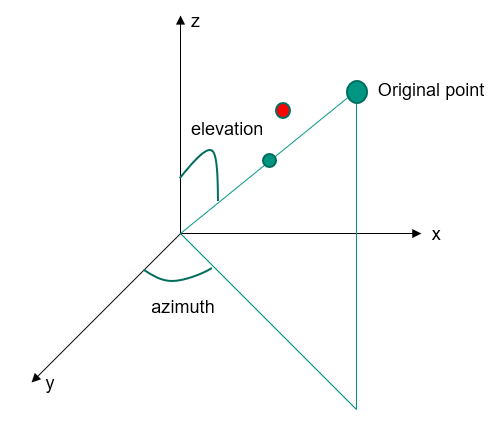
\includegraphics[scale=0.5]{Graphics/Adjustment.png}
\caption{LiDAR Point Coordinate System}
\label{fig:Adjustment}
\end{figure}

\section{Drop Critical Points}

\begin{enumerate}
 \item \textit{Critical Features}
 
PointPillars\cite{lang_pointpillars_2019} uses simplified PointNet\cite{qi_pointnet_2017}, which is called Pillar Feature Net. Pillar Feature Net's first two step is import for definition of critical features. The first step is to stack points into pillars, the second step is to get learned features in each pillar. The learned features is defined as critical features.
\begin{figure}[!htbp]
\centering
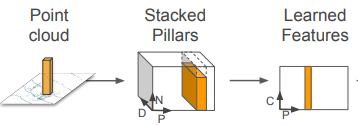
\includegraphics[scale=1]{Graphics/Pillar Feature Net.png}
\caption{Part of Pillar Feature Net}
\label{fig:Pillar Feature Net}
\end{figure}
\item \textit{Critical Points}

Definition critical points with two criterion:

1. Critical point in each pillar is the point with maximum critical feature value. 

2. Critical point is the point that has most critical features.

In Figure 4.4, cells with critical features are pinpointed in colored background. In the whole table, 10 is the maximal critical feature value, and it's located at the third row, so this point is a critical point from first criterion. When counting the number of critical features, the fourth row has four colored cells, showing it has most features than other points. So, this point is a critical point based on second criterion.
\begin{figure}[!htbp]
\centering
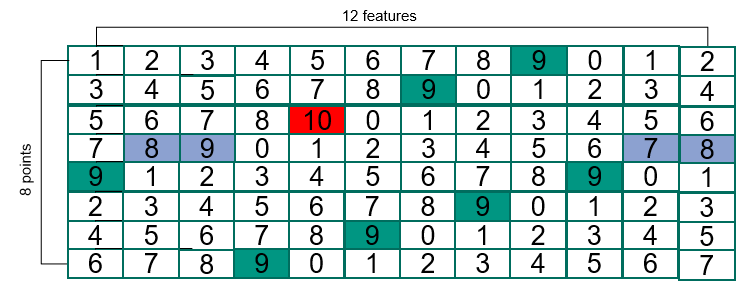
\includegraphics[scale=0.5]{Graphics/Critical Points.png}
\caption{Pseudo Process of Catching Critical Features}
\label{fig:Critical Points}
\end{figure}
\end{enumerate}

\section{Points Perturbation and Points Drop}

\begin{enumerate}
\item\textit{Points Perturbation and Points Drop methods}

1. Points Perturbation on different features: intensity \(r\), \(xyz\) coordinates, and the combination of \(xyz\) coordinates and intensity \(r\).
2. Points randomly drop: the number of dropping points rely on the total number of points.
 \item \textit{Benchmark}
 To evaluate the robustness, rPC, which is the relative performance under point cloud changes, is used. RPC is the ratio of mPP and \(P_{clean}\):
\begin{center}
          \(rPC = \frac{mPC}{AP_{clean}} \)
\end{center}
\(AP_{clean}\) is the average precision of the detection model under clean dataset, and mPC is the mean value of average precision of detection under benchmark datasets:
\begin{center}
          \(mPC = \frac{1}{N_{C}}\sum_{c=1}^{N_{C}}\sum_{s=1}^{N_{S}}{AP_{C,S}} \)
\end{center}
\({P_{C,S}}\): performance evaluated on data changed with changes C with perturbation and drop points under severity level S

\({N_{C}}\): number of changes, including different methods

\({N_{S}}\) :severity levels

\end{enumerate}

\section{Adverse Weather Point Clouds Simulation}

\begin{enumerate}
 \item \textit{Simulate Methods}
 
 1. Add gaussian noise perturbation.

2. Drop points randomly.

3. Add points surround cluster and ground points. Use RANSAC to segement ground points of lidar point clouds and then get clusters with DBSCAN. Random pick the some points in cluster and ground points to do the gaussian noise perturbation and then add the perturbated points to the original points as the addition of noise points.
 
 \item \textit{Evaluation Metric: Weather Classification} 
 
 Vargas et.al\cite{vargas_rivero_weather_2020} have shown, use simple statistic parameters of point clouds: standard deviation and mean value of \(x\) coordinates and mean and standard deviation of echo-pulse width, which is intensity, etc. 13 parameters as input for a weather classifier.
 \item \textit{Evaluation Metric: Weather Points Semantic Segmentation}
 
 
 Evaluate the performance of simulation, weather point semantic segementation network is introduced. As the figure 6 shown, the DENSE Dataset labeled each point cloud with a weather category, which is adverse weather consists of rain and fog. Heinzler et.al \cite{heinzler_cnn-based_2020} proposed WeatherNet training on DENSE Dataset. His results is shown in Table 4.1
 \begin{table}[h!]
  \begin{center}
    \caption{Training Results on DENSE Dataset}
    \begin{tabular}{|c|c|c|c|} % <-- Alignments: 1st column left, 2nd middle and 3rd right, with vertical lines in between
      \hline
      \multirow{2}{*}{Methods} & \multicolumn{3}{c|}{Weather Class}\\
    \cline{2-4}
       &\textbf{Clean(mIOU)} & \textbf{Rain(mIOU)}& \textbf{Fog(mIOU)}\\
      \hline
      WeatherNet & 93.35 & 90.92&88.81\\
      Cylinder3D & 98.91 & 94.61&91.63\\
      \color{blue}
      Delta & \color{blue}+5.56 & \color{blue}+3.69&\color{blue}+2.28\\
    \hline
    \end{tabular}
  \end{center}
\end{table}
Cylinder3D\cite{zhu_cylindrical_2020} performs well in Semantic KITTI\cite{behley_semantickitti_2019}, which is an object semantic datasets. 
\end{enumerate}
